% Online实机吡啶示例；由主控插入第7章适当位置。
% 仅以LaTeX矩形裁切原JPEG，不修改、拼接或重绘像素。
\begin{figure}[H]
\centering
% 原图3024×1758；参数范围(710,735,2315,1585)，1605×850，122mm约334ppi。
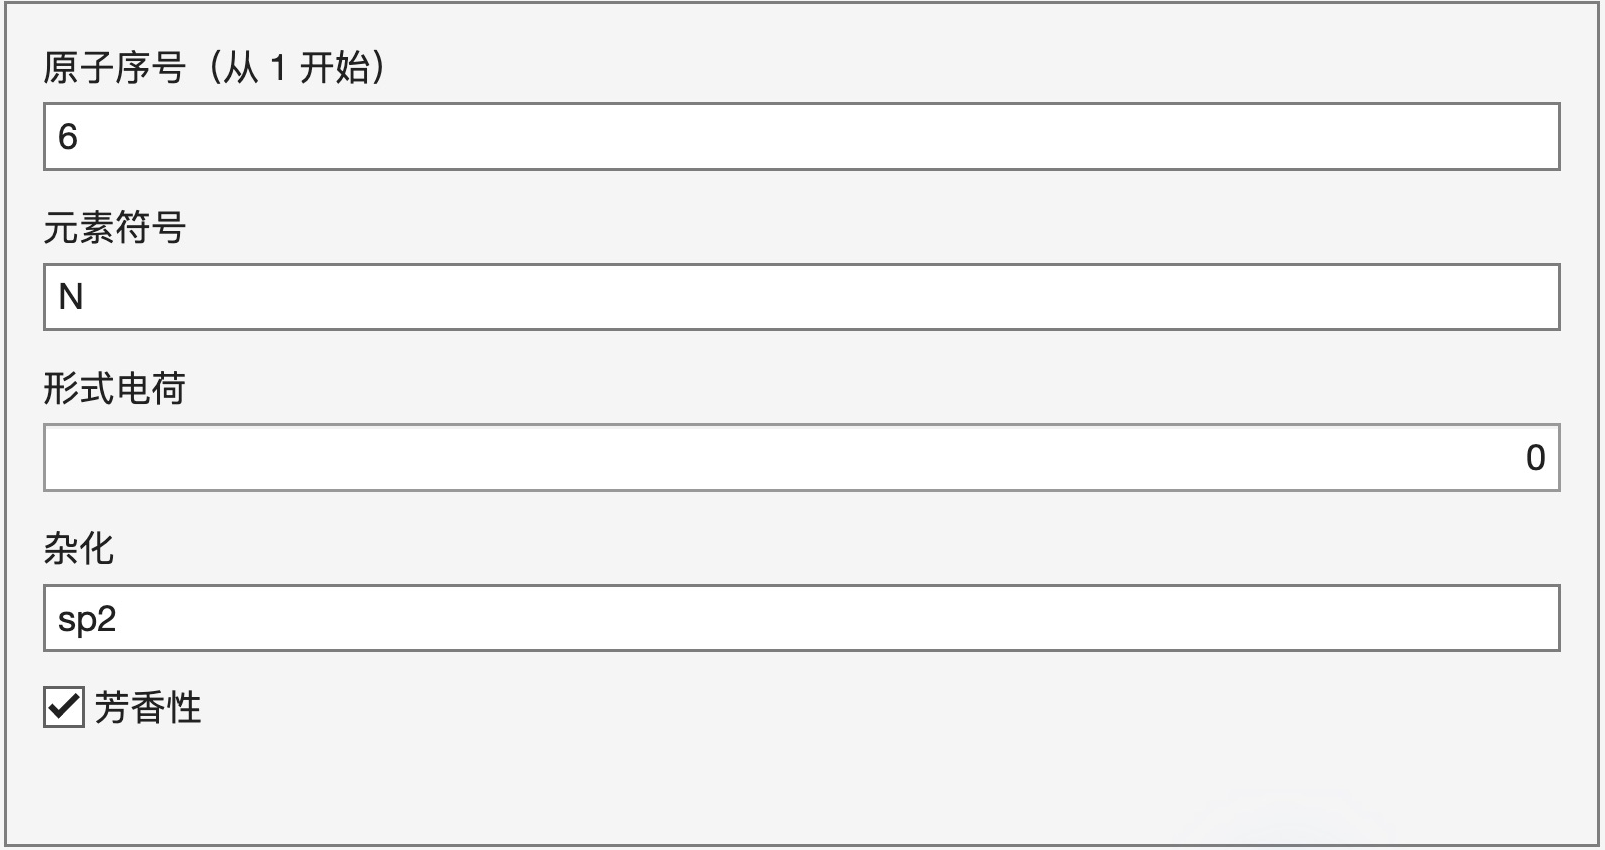
\includegraphics[width=\linewidth]{publication-assets/crop-f99354db0f163eccfd81.png}
\par\vspace{2mm}
% 同一原图的独立预览提示范围(700,1615,1520,1670)，820×55；排除右侧指针。

\includegraphics[width=80mm]{publication-assets/crop-8ce96edd826deccee006.png}
\caption{Online中把环上第6个原子替换为氮的实际参数：元素为N，形式电荷为0，杂化为\ui{sp2}，勾选\ui{芳香性}。下方为同一次操作的预览提示；此时仍需单击应用提交。}
\label{fig:pyridine-chemistry}
\end{figure}
